% Analysis section
In this section we will outline the process used for each clustering method, and the process of selecting colours for clustering.

\subsection{Colour Selection}

An aim of this work was to help astronomers determine which filters were best at identifying different types of objects in a survey. 
Since the average survey is limited to four filters, different combinations of four filters were used to construct colours for clustering. 
Due to the large number of filters available in the ERS data, the combinations had to be narrowed down to a reasonable set.
Two types of colour combinations were created.

\subsubsection{Broad Band Combinations}

\textbf{PB: Should we explain what we hope to find in these combos?}

The first type of combination was comprised of the broad band filters: F336W (U), F438W(B), F555W(V), and F814W(I).
The F225W (UVW) filter was not included in this set as it is not a standard filter found in most surveys.
Additionally, the $U - I$ colour was not used in the analysis because it was determined that this colour was not physically meaningful.
This is because it is unlikely that an object would emit a detectable reading in both these bands due to their distance from one another in wavelength.
The $B - V$ colour was not used in the broad band analysis, instead in the narrow band analysis.
Using the four filters listed above, the broad band colour combinations created can be found in Table~\ref{tab:BBcolours}.
These combinations were created in order to remove any obvious correlation between the colours that could occur by the inclusion of the same band in both colours.

\begin{table*}
\centering
\caption{Broad band colour combinations and the number of objects detected in each colour, and in each combination, with uncertainties less than $0.2$.}
\label{tab:BBcolours}
\begin{tabular}{lllllll}
\hline\hline
Colour 1 & Objects & Mean Uncertainty & Colour 2 & Objects & Mean Uncertainty & Combined Objects \\
\hline
$U - B$ &  33523 & 0.1606 mag & $V - I$ &  57935 & 0.1334 mag & 28931\\
$U - V$ &  33692 & 0.1429 mag & $B - I$ &  41413 & 0.1590 mag & 28931\\
$B - V$ &  48660 & 0.1456 mag & $ - $ & $ - $ & $ - $ & $ - $ \\
\hline
\end{tabular}
\end{table*}

\subsubsection{Narrow Band Combinations}

\textbf{PB: Should we explain more about why we choose to do Broad - Narrow? And what we hope to find in these combos?}

The second set of combinations included the narrow band filters: F373N ($O_{2}$), F487N ($H\beta$), F502N ($O_{3}$), F657N ($H\alpha$), and F673N ($S_{2}$).
In addition, the broad band F225W (UVW) was included in this set to ensure its data was included in the analysis. 
Colours were created with the narrow bands by pairing them with the broad bands that covered them in wavelength space.
These colours were created in order to reduce the number of possible combinations that could be used for analysis.
The second colour in each combination was created from two broad bands that did not overlap the first colour in wavelength space.
Table~\ref{tab:NBcolourcombos} lists the narrow band colour combinations used for analysis.
The number of objects in the narrow band combination, with the exception of the $H\alpha$ band, is significantly lower than the broad band combinations.
These combinations were useful for analysis as their distributions were not as dense as the broad bands, and the clustering algorithms were able to detect interesting structure within them.

\begin{table*}
\centering
\caption{Narrow band colour combinations and the number of objects detected in each colour, and in each combination, with uncertainties less than $0.2$.}
\label{tab:BBcolours}
\begin{tabular}{lllllll}
\hline\hline
$Narrow - Broad$ & Objects & Mean Uncertainty & $Broad - Broad$ & Objects & Mean Uncertainty & Combined Objects \\
\hline
$UVW - U$ &  14977 & 0.1539 mag & $B - V$ &  48660 & 0.1456 mag & 14943 \\
$ - $ & $ - $ & $ - $ & $B - I$ &  41413 & 0.1590 mag & 14095 \\
$ - $ & $ - $ & $ - $ & $V - I$ &  57935 & 0.1334 mag & 14098 \\
\hline
$U - O_{2}$ & 8675 & 0.1504 mag & $B - V$ &  48660 & 0.1456 mag & 8657 \\
$ - $ & $ - $ & $ - $ & $B - I$ &  41413 & 0.1590 mag & 8558 \\
$ - $ & $ - $ & $ - $ & $V - I$ &  57935 & 0.1334 mag & 8559 \\
\hline
$B - H\beta$ & 13269 & 0.1493 mag & $V - I$ &  57935 & 0.1334 mag & 13147 \\
\hline
$O_{3} - V$ & 14644 & 0.1418 mag & $U - B$ &  33523 & 0.1606 mag & 13390 \\
\hline
$H\alpha - I$ & 59465 & 0.1495 mag & $U - B$ &  33523 & 0.1606 mag & 28920 \\
$ - $ & $ - $ & $ - $ & $U - V$ &  33692 & 0.1429 mag & 29060 \\
$ - $ & $ - $ & $ - $ & $B - V$ &  48660 & 0.1456 mag & 41317 \\
\hline
$S_{2} - I$ & 25185 & 0.1535 mag & $U - B$ &  33523 & 0.1606 mag & 14577 \\
$ - $ & $ - $ & $ - $ & $U - V$ &  33692 & 0.1429 mag & 14586 \\
$ - $ & $ - $ & $ - $ & $B - V$ &  48660 & 0.1456 mag & 18882 \\
\hline
\end{tabular}
\end{table*}

\subsubsection{Number of Dimensions}
Due to the high number of bands available in the ERS data, the number of dimensions available to cluster was very high.
Limiting the number of band combinations through the system outlined above helped reduce the number of dimensions.
However, in addition to the two dimensional combinations, clustering in three dimensions was investigated.
Three dimensional colour combinations were created based on the combinations listed in Table~\ref{tab:BBcolours} and Table~\ref{tab:NBcolourcombos}.
In the broad band combinations, three dimensional colour spaces were created by making colours with a common band, either B or V.
These bands were selected in order to avoid creating the $U - I$ colour.
\textbf{PB: Not sure if this next sentance explains why we chose to use a common band clearly. Just trying to say that the colours could be subtracted to transform back into the two dimensional space.}
A common band was used in all colours in order to create a three dimensional space that of colours that could be transformed back into the original two dimensional space. 

In the narrow band combinations, the three dimensional colour spaces were created by making colours with the narrow band common between them.
Similar to the broad band spaces, these combinations could be transformed into the original two dimensional space, and act as an extension of the two dimensional distribution.

Clustering in three dimensions increased the complexity of the distribution, creating more information for the clustering algorithms to use.
However, limiting the dimensionality of the problem to three allowed the analysis to stay within the constraints of a common survey.
A space of up to 45 dimensions could have been created, but that space would not be reasonable for the analysis of a common survey.

\subsection{Clustering Process}
Clustering was performed using all methods for each colour combination. 
The following process allowed the investigation of the effect of all paramters on each clustering technique, allowing the selection of an optimal clustering.

\subsubsection{Meanshift}
Mean-Shift clustering was performed first by estimating the bandwidth paramter with the $estimate-bandwidth$ function in $scikit-learn$.
Following the initial clustering, a the bandwidth was varried and the clustering was performed again with bandwidth values on intervals of $\pm 0.1$ from the estimated bandwidth value.
Varying the bandwidth uncovered a combinations sensitivity to the parameter.
If a combination was very sensitive to bandwidth, then the number of clusters that meanshift would predict would vary greatly over a small range of bandwidth values.
This type of combination usually resulted in poor segmentation, as the algorithm would not converge on a number of clusters. 
However, sensitivity could also be the result of the starting bandwidth estimate.
If the original estimate was in an unstable bandwidth interval, then the hierarchy would reflect that, and the testing of multiple bandwidth values could result in convergence.

\subsubsection{Affinity Propagation}
Affinity Propagation clustering was performed after meanshift by setting the preferences to 10\% of the number of objects in the data set, and setting the damping factor to $0.95$.
Similar to the Meanshift process, the clustering was repeated by varrying the damping factor and preference value to determine the effect of each parameter.
After initial tests of Affinity Propagation, it was determined that this clustering method was not effective for the dataset.
Due to the number of computations required for the calculation of the messages passed between points on each iteration, the algorithm was very sensitive to the input parameters, and did not produce meaningful clusterings.
The algorithm is effective for small and medium sized datasets, and was able to create some reasonale clusters for the $U - O_{2}$ colour combinations.
However, as the number of objects increased, the sensitivity to parameter selection became very high, and the number of clusters produced exceed 100 for only 20 000 objects clustered.
After multiple clusterings, no systematic way of determine the correct number of clusters was determined, and the algorithm was no longer used.

\subsubsection{K-Means}
K-Means clustering was performed last.
The first two clusterings were performed using the number of clusters determined from the initial clusterings by Meanshift and Affinity Propogation until it was discontinued.
Next, K-Means was performed with $K = \pm 4$ from the original clustering.
This method of clustering was similar to the Meanshift approach, as it showed the results of different values of $K$.
K-Means was the most efficient algorithm of the three. It produced clusterings quickly, and always produced clusters of reasonable size.

\subsection{Selecting the Optimal Clustering}
In order to determine the optimal clustering, a series of processes were used.
For each clustering, a variety of metrics and statistics were calculated to measure the compactness and isolation of each cluster.
Additionally, a process was developed for determining the relationships between a variety of parameters and the optimal clustering.
The performance of the algorithms were directly related to the parameters used as input, and those relationships were critical for choosing the correct clustering.
\subsubsection{Silhouette Score}
The silhouette score is a metric used to describe the compactness of a cluster in a given clustering and is calculated as an average of all samples in a clustering.  
The silhouette score is given by:
\begin{equation}
\label{eq:ss}
Silhouette Score = \frac{b - a}{\textit{max}\big(a, b\big)}
\end{equation}
where $a$ is the mean intra-cluster distance, and $b$ is the distance between a point and the nearest cluster that point is not a member of.
In addition to the average score of the clustering, the average score for each cluster within the clustering was computed.
The cluster score determines what is driving the average score, and uncovers which clusters are most compact.

\subsubsection{Cluster Statistics}
Various statistics were calculated for each cluster within a clustering to help describe the similarity between the objects in a given cluster.
The standard deviation and average colour was calculated for each colour and each cluster within a clustering. 
These metrics describe the distribution of the objects in the colour-colour space within a cluster. 
Clusters that had large standard deviations were viewed as too dissimilar to be a meaningful cluster, and the clustering parameters were changed or the clustering was removed. 
Clusters whose averages and medians were not close were also discredited. 

The fractional sizes of each cluster were also calculated.
This metric describes the distribution of objects between clusters, and provided a complete way to evaluate a given clustering. 
If a clustering segmented the objects into a large cluster followed by several smaller ones, the clustering was investigated further, as this segmentation could mean one of two things. 
This type of clustering could be a result of the identification of interesting objects, in which case the clustering algorithm was able to identify the objects and place them in the same cluster.
However, this type of clustering could also be a result of the underlying distribution of the data, as the clustering techniques are largely drawn to areas of high density.
If this is the case, the clustering only created the smaller clusters as a result of the parameters imposed on the clustering.

\subsubsection{Parameter Relationships}
In addition to metrics, the relationships between various metrics were investigated to determine the optimal clustering.
Figure~\ref{fig:sscore} shows the relationship between the silhouette score and the number of clusters imposed on the data for each type of clustering. 
The optimal number of clusters is found where the relation flattens.
For K-Means, this point is between 5-10 clusters.

\begin{figure}[H]
\centering
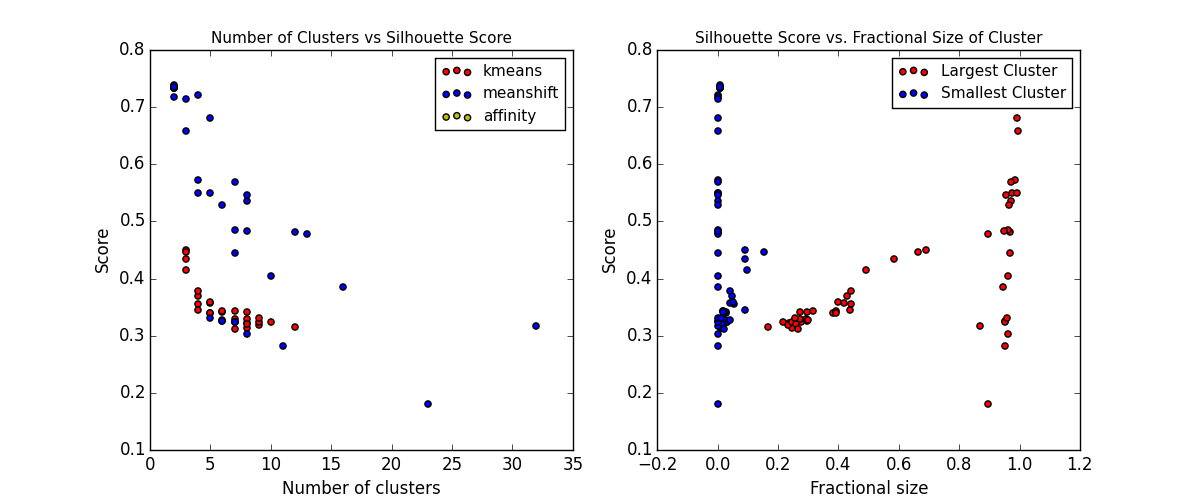
\includegraphics[width=\linewidth]{figs/silhouette_score_relation}
\caption{Distribution of the silhouette score as a result of the number of clusters imposed. The \textit{blue} points are the scores of Mean-Shift clustering, \textit{red} points are scores of K-Means, and \textit{yellow} points are scores of AP.}
\label{fig:sscore}
\end{figure}

The Mean-Shift scores do not follow a similar distribution as K-Means, as the accuracy of Mean-Shift is more directly related to the bandwidth parameter, seen in Figure~\ref{fig:bwscore}.
The optimal Mean-Shift clustering was chosen by finding the bandwidth where the relation between the bandwidth and number of clusters reached an elbow, which was usually between 3 - 5 clusters.

\begin{figure}[H]
\centering
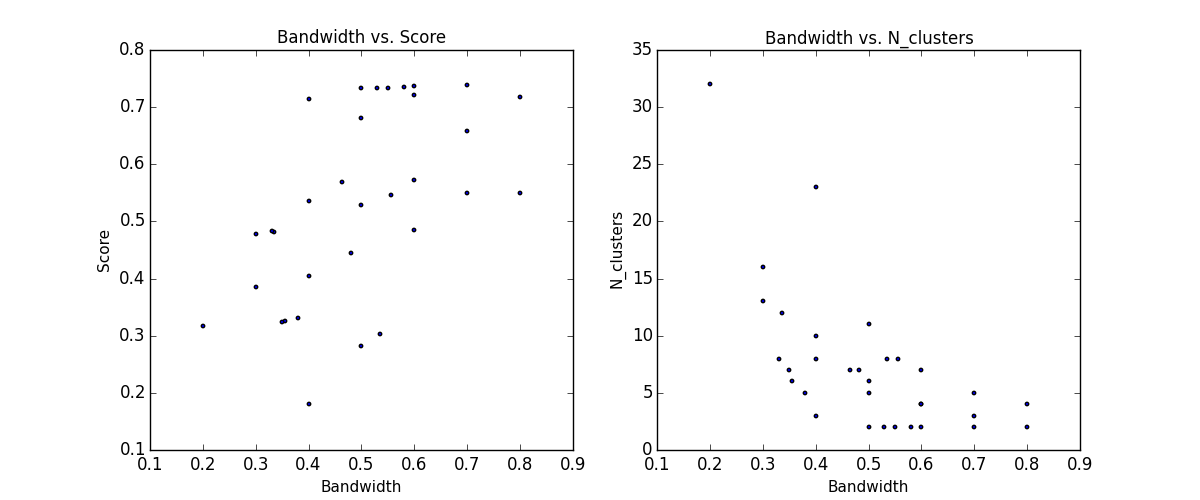
\includegraphics[width=\linewidth]{figs/meanshift_parameters}
\caption{Distribution of the silhouette score as a function of bandwidth, and the distribution of the number of clusters as a function of bandwidth.}
\label{fig:bwscore}
\end{figure}
